\documentclass[12]{article}

%% packages used
\usepackage{fullpage}
\usepackage{graphicx}
\usepackage{setspace}
\usepackage{hyperref}

%% packages not used
% \usepackage{ifthen}
% \usepackage{verbatim}
% \usepackage{pdfpages}




\title{Quantitative Methods for: Socialist Indoctrination in Venezuela}
\author{Ragan}

\begin{document}

\maketitle

\doublespace

\section{Literature}



\section{Methods}
The quantitative text analysis was preformed on the pre-Chavez and post-Chavez textbook sets. The textbooks were all in PDF format when we received them. The post-Chavez textbooks we already in machine readable form and we were able to directly read in those files for our text analysis. The pre-Chavez textbooks were also PDFs, but the text in these PDFs were not machine readable. We attempted to use various methods for converting the PDFs to a machine readable form using optical character recognition (OCR). The results from these attempts were always poor. In order to ensure that all the text from both textbooks sets was available for analysis we used the website Upwork.com to hire several Venezuelans to transcribe the PDFs to plain text for us. Once the pre-Chavez textbooks were transcribed we had five machine readable textbooks (Grade 1 - Grade 5) from both the pre-Chavez and post-Chavez eras. For both sets of textbooks the following steps were taken:\footnote{All of the R code used in the text analysis is available as an R Package that can be installed an run using the free R statistical language. The package can be found on GitHub at \url{https://github.com/robiRagan/prePostChavezTextbooks}}

\begin{enumerate}


\item Extract all words from the textbook and store them along with the page number the word was located on.
	
	\begin{enumerate}
	\item The raw text from the PDF or Text file for a single textbook is read in and stored as an object. Here we will refer to this as \textbf{rawTextbookObject}. \label{beginTokenize}
	
	\item \textbf{rawTextbookObject} is then split with each page in the original text becoming its own data frame. Here we will refer to these as \textbf{rawPageDataFrames}.

	\item The \textbf{rawPageDataFrames} are stored as a single R list. With each page being a data frame that is one element of the R list. Here we will refer to this list as \textbf{rawPagesList}.

	\item For each page the raw text is tokenized. With each word receiving its own row in the first column of the data frame. The data frames will now be referred to as \textbf{tokenizedPageDataFrames} and the list storing all the data frames will be called \textbf{tokenizedPagesList}. 
	
	\item The second column in each of the \textbf{tokenizedPageDataFrames} contains the page number that each word appeared on. At this stage, each page has been converted to a two column data frame. The first column contains all the words on the page and the second column contains the page number the word appeared on. All of the \textbf{tokenizedPageDataFrames} are stored in an R list, \textbf{tokenizedPagesList}.

	\item All of the \textbf{tokenizedPageDataFrames} in \textbf{tokenizedPagesList} are merged into one data frame that contains all of the words in the textbook as the first column, and the page the word was found on as the second column. Here we will refer to this as \textbf{oneTokenizedTextbookDataFrame}.\label{endTokenize}
	
	\item Steps \ref{beginTokenize} through \ref{endTokenize} are run for each of the five textbooks in a set.
	\end{enumerate}

\item Add the grade level to the data frame for each textbook and combine the five data frames into one data frame.

	\begin{enumerate}
	
	\item A third column is added to each \textbf{oneTokenizedTextbookDataFrame} that contains the grade level for the textbook. 
	
	\item The five \textbf{oneTokenizedTextbookDataFrame}s are all combined into one data frame. 
	
	\end{enumerate}


\end{enumerate}



\begin{itemize}
	\item 
\end{itemize}



\section{Findings}



\begin{figure}[h!]
  \centering
  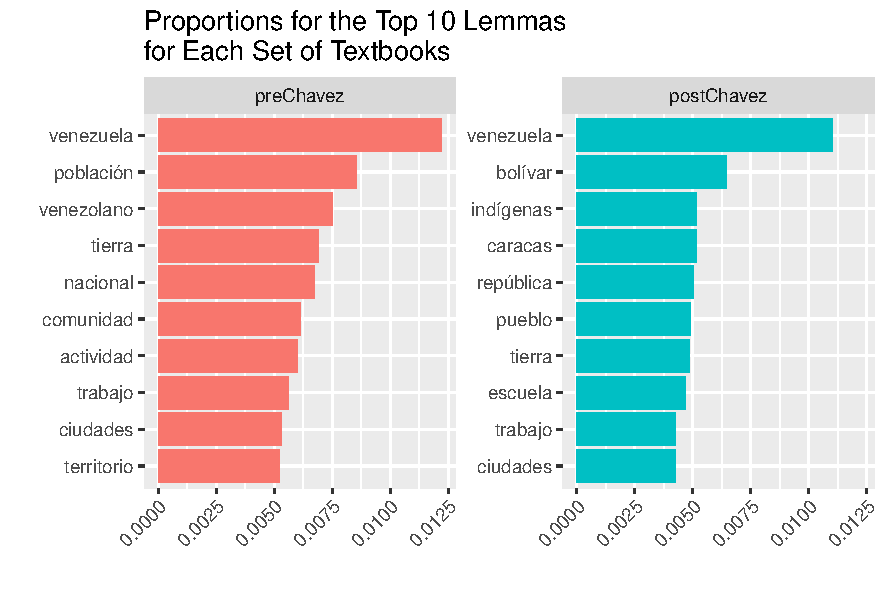
\includegraphics[width=4.5in]{images/top10AllLemmasProp}\\
  \caption{caption}
\end{figure}






\newpage
\bibliography{bib.bib}
\bibliographystyle{apsr}


\end{document}


# Generic Code to Insert Figures:

%\begin{figure}[h!]
%  \centering
%  \includegraphics[width=4in]{"filename"}\\
%  \caption{caption}
%\end{figure}